\documentclass[12pt,a4paper]{article}
\usepackage[utf8]{inputenc}
\usepackage[spanish]{babel}
\usepackage{graphicx}
\usepackage{hyperref}
\usepackage{float}
\usepackage{amsmath}
\usepackage[margin=2.5cm]{geometry}

\begin{document}
% Portada
\begin{titlepage}
    \centering
    \vspace*{1cm}
    
\includegraphics[width=0.8\linewidth]{espe.png}\\[0.5cm]
    
    \Large \textbf{Departamento de Ciencias de la Computación}\\
    \large \textbf{Universidad de las Fuerzas Armadas - ESPE}\\[0.5cm]
    
    \Huge \textbf{Cuaderno de clases de la asignatura de Ingeniería de Seguridad de Software}\\[0.3cm]
    \Large \textbf{Parcial No. 1}\\[0.8cm]
    
    \textbf{Nombres:}\\
    Yeshua Amador Chiliquinga Amaya\\[0.3cm]
    
    \textbf{Carrera / Asignatura:} Ingeniería de Software / Ingeniería de Seguridad de Software\\
    \textbf{NRC:} 2540\\
    \textbf{Nombre del profesor:} Walter Fuertes, PhD\\[0.5cm]
    
    \textbf{Fecha de presentación:} 24 de mayo del 2025\\[1cm]    
    \vfill
\end{titlepage}
% Índice de contenido

\tableofcontents
\newpage

\section{Clase 1 - 17 de Abril 2025: Introducción a la Ingeniería de Seguridad de Software}
\subsection{Objetivos de Aprendizaje}
\begin{enumerate}
    \item Motivación
    \item Presentación
    \item Syllabus
    \item Unidad 1
    \begin{enumerate}
        \item Introducción a la Ciberseguridad
    \end{enumerate}
\end{enumerate}

\subsection{¿Por qué de la asignatura?}
\textbf{Ciudadanía digital}

Cuando Julian Assange estaba en la embajada recibimos más de 4 millones de ataques.

\subsection{Syllabus}
\subsubsection{Unidad 1: Introducción a la seguridad de la información}
\begin{itemize}
    \item Seguridad de la información
    \item Ciberseguridad
    \item Componentes
    \begin{itemize}
        \item Amenazas
        \item Vulnerabilidad
        \item Riesgo
        \item Incidentes
    \end{itemize}
    \item Tríada CID (ISO 27000)
    \begin{itemize}
        \item Confidencialidad
        \item Integridad
        \item Disponibilidad
    \end{itemize}
    \item Herramientas tecnológicas para garantizar la CID
    \item Análisis de amenazas y vulnerabilidades
    \item Requerimientos funcionales para implementación de tecnologías de ciberseguridad
\end{itemize}

\subsection{Unidad 2: Mecanismos de seguridad}
\begin{itemize}
    \item Criptografía
    \begin{itemize}
        \item Simétrica
        \item Asimétrica
    \end{itemize}
    \item Funciones Hash aplicadas al software
    \item Firma digital y certificados digitales
    \item Autenticación vs Identificación
    \item Seguridad Física
    \item Protocolos Criptográficos
\end{itemize}

\subsection{Unidad 3: Seguridad de Redes y Aplicaciones}
\begin{itemize}
    \item Seguridad de Redes
    \begin{itemize}
        \item Perimetral
        \item En profundidad
        \item Multinivel
    \end{itemize}
    \item IPS/IDS
    \item Firewall
    \item Seguridad de aplicaciones en internet
    \item OWASP Top 10
    \item SGSI (Sistema de Gestión de Seguridad de la Información)
    \begin{itemize}
        \item Lógica
        \item Física
        \item Legal
        \item Procedimental
    \end{itemize}
    \item Temas adicionales
    \begin{itemize}
        \item Blockchain
        \item Seguridad criptográfica
        \item Computación en la nube
    \end{itemize}
    \item Seguridad en la nube
    \item Deep web
    \item IoT (Internet de las Cosas)
\end{itemize}

\subsection{Plataforma (topología) experimental}
\begin{itemize}
    \item Entorno controlado
    \item COIP (Código Orgánico Integral Penal)
    \item Delitos informáticos tipificados
\end{itemize}

\textbf{VNE:} Virtual Network Environment

\subsection{Referencias Bibliográficas}
\begin{itemize}
    \item Norma ISO 27000
    \item Código Orgánico Integral Penal (COIP)
    \item Material del curso - Ing. Walter Fuertes, PhD
\end{itemize}

\section{Clase 2 - 24 de Abril 2025}
\subsection{Tríada CID}
La tríada CID (Confidencialidad, Integridad, Disponibilidad) es un modelo fundamental en seguridad de la información que establece los tres pilares principales de la protección de datos.

\subsection{Delito Informático (COIP)}
\begin{itemize}
    \item Todo acto malicioso en contra de las personas, empresas y estado utilizando herramientas informáticas en el ciberespacio.
    \item Incluye actividades como acceso no autorizado, interrupción de servicios, fraude electrónico, entre otros.
\end{itemize}

\subsection{Ciber-atacantes}
\begin{itemize}
    \item \textbf{Insiders}: Atacantes que vulneran desde dentro de la organización.
    \item \textbf{Spammers}: Distribuyen correos no deseados o maliciosos.
    \item \textbf{Piratas telefónicos}: Se introducen en las líneas telefónicas para realizar llamadas sin costo.
    \item \textbf{Geeks}: Personas con amplios conocimientos técnicos.
    \item \textbf{Hackers de sombrero blanco/negro}: Éticos vs. malintencionados.
\end{itemize}

\begin{figure}[H]
    \centering
    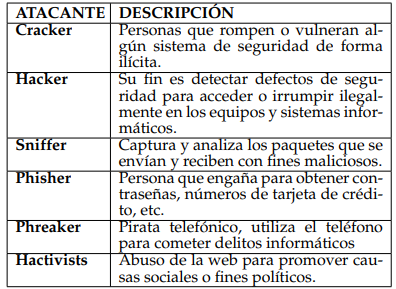
\includegraphics[width=0.8\textwidth]{atacante_descripcion.png}
    \caption{Descripción de tipos de ciber-atacantes}
    \label{fig:atacantes}
\end{figure}

\subsection{Ciber-ataques}
\begin{itemize}
    \item \textbf{Ingeniería Social}: Aprovechan la ingenuidad de los usuarios (capa 8 del modelo OSI).
    \item \textbf{DoS/DDoS}: Ataques de denegación de servicio.
    \item \textbf{Aplicaciones Web}: Vulnerabilidades según OWASP.
    \item \textbf{Ciber-terrorismo}
    \item \textbf{Ciber-espionaje}
    \item \textbf{Ciber-sabotaje}
\end{itemize}

\subsection{Ciber-defensa}
Para contrarrestar las amenazas se necesitan Ciber-soldados o COCICIBER (Comando de Ciberdefensa). La ciberdefensa utiliza la ciberseguridad en tres niveles:
\begin{itemize}
    \item \textbf{Pasiva}: Medidas preventivas.
    \item \textbf{Activa}: Detección y respuesta.
    \item \textbf{Ofensiva}: Contramedidas activas.
\end{itemize}

\subsection{Tipos de amenazas}
\begin{itemize}
    \item \textbf{Ataques de fuerza bruta}
    \item \textbf{Man in the Middle (MitM)}
    \item \textbf{Malware}:
    \begin{itemize}
        \item Troyanos
        \item Botnets (redes de equipos zombis)
        \item Virus
        \item Gusanos
        \item Insectos
    \end{itemize}
    \item Ciberarmas
\end{itemize}

\subsection{Gestión del Tiempo}
\begin{itemize}
    \item Importancia de la gestión eficiente del tiempo
    \item Distribución recomendada:
    \begin{itemize}
        \item Perfección intelectual
        \item Salud
        \item Actividad Física
        \item Entretenimiento
        \item Tiempo para la familia
        \item Trabajo
        \item Perfeccionamiento Espiritual
    \end{itemize}
\end{itemize}

\section{Clase 3 - Herramientas Tecnológicas para la Seguridad del Software}
\subsection{Objetivos de Aprendizaje}
\begin{itemize}
    \item Comprender la arquitectura jerárquica de seguridad en redes
    \item Identificar y clasificar herramientas tecnológicas según su función
    \item Analizar mecanismos de seguridad en diferentes niveles de red
    \item Evaluar herramientas de prevención, detección, cifrado y mitigación
\end{itemize}

\subsection{Arquitectura de Seguridad en Redes}
La seguridad en redes se implementa a través de una arquitectura jerárquica centralizada con diferentes niveles de acceso y control:

\subsubsection{Niveles de Seguridad}
\begin{enumerate}
    \item \textbf{Nivel de Cliente/Acceso}
    \begin{itemize}
        \item Perfil de usuario
        \item Claves de acceso
        \item Software de seguridad local
    \end{itemize}
    
    \item \textbf{Nivel de Servidor}
    \begin{itemize}
        \item Gestión de cuentas
        \item Firewalls (iptables, ufw)
        \item Sistemas de detección/prevención de intrusiones (IDS/IPS)
    \end{itemize}
    
    \item \textbf{Nivel de Red (Core)}
    \begin{itemize}
        \item Enrutamiento seguro
        \item Filtrado de paquetes
        \item NAT (Traducción de Direcciones de Red)
    \end{itemize}
\end{enumerate}

\begin{figure}[H]
    \centering
    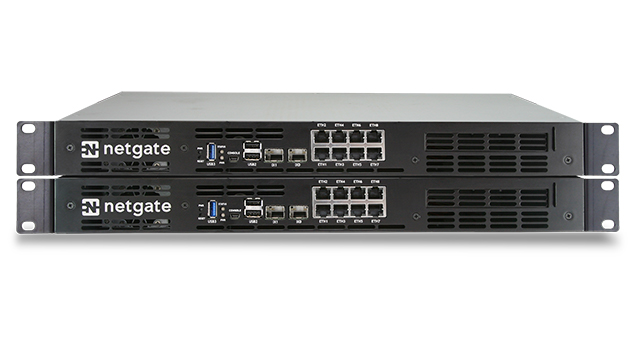
\includegraphics[width=0.8\textwidth]{netgate.png}
    \caption{Arquitectura de seguridad en redes con Netgate}
    \label{fig:netgate}
\end{figure}

\subsection{Herramientas de Seguridad por Categoría}

\subsubsection{Seguridad Inalámbrica}
\begin{itemize}
    \item \textbf{Protocolos de Seguridad}:
    \begin{itemize}
        \item WEP (Wired Equivalent Privacy)
        \item WPA/WPA2 (Wi-Fi Protected Access)
        \item EAP (Extensible Authentication Protocol)
    \end{itemize}
    \item \textbf{Dispositivos}:
    \begin{itemize}
        \item Puntos de Acceso Inalámbrico (WAP)
        \item Controladores de Redes Inalámbricas
    \end{itemize}
\end{itemize}

\subsubsection{Seguridad Perimetral}
\begin{itemize}
    \item \textbf{Firewalls}:
    \begin{itemize}
        \item pfSense
        \item ClaroOS
        \item Firewalls de Próxima Generación (NGFW)
    \end{itemize}
    \item \textbf{Sistemas de Gestión de Amenazas Unificadas (UTM)}
    \item \textbf{Servidores Proxy}
\end{itemize}

\subsubsection{Monitoreo y Análisis}
\begin{itemize}
    \item \textbf{Wireshark}: Análisis de tráfico de red
    \item \textbf{Nmap}: Mapeo de red y escaneo de puertos
    \item \textbf{SIEM}: Gestión de Eventos e Información de Seguridad
    \item \textbf{Metasploit}: Marco de pruebas de penetración
\end{itemize}

\subsection{Clasificación de Herramientas}
\begin{table}[H]
    \centering
    \begin{tabular}{|l|l|l|}
    \hline
    \textbf{Tipo} & \textbf{Herramientas} & \textbf{Propósito} \\ \hline
    Prevención & Firewalls, UTM, NGFW & Bloquear amenazas antes de que ingresen \\ \hline
    Detección & IDS/IPS, SIEM & Identificar actividades sospechosas \\ \hline
    Cifrado & VPN, WPA3, SSL/TLS & Proteger la confidencialidad de los datos \\ \hline
    Mitigación & Balanceadores de carga, DDoS Protection & Reducir el impacto de los ataques \\ \hline
    \end{tabular}
    \caption{Clasificación de herramientas de seguridad}
    \label{tab:herramientas}
\end{table}

\subsection{Herramientas Avanzadas}
\begin{itemize}
    \item \textbf{APT (Amenazas Persistentes Avanzadas)}: Tácticas sofisticadas para atacar objetivos específicos
    \item \textbf{Metasploit Framework}: Para pruebas de penetración y desarrollo de exploits
    \item \textbf{Nmap}: Herramienta de descubrimiento de red y auditoría de seguridad
\end{itemize}

\subsection{Conclusión}
La seguridad del software requiere un enfoque en capas que combine múltiples herramientas tecnológicas. Desde la protección perimetral hasta el monitoreo continuo, cada capa juega un papel crucial en la defensa contra amenazas cibernéticas. La selección e implementación adecuada de estas herramientas, junto con prácticas de seguridad sólidas, son fundamentales para mantener la integridad, confidencialidad y disponibilidad de los sistemas de información.

\subsection{Próximos Pasos}
\begin{itemize}
    \item Investigar sobre el Congreso Internacional de Ciencia y Tecnología ESPE 2025
    \item Desarrollar un artículo científico siguiendo el formato Springer
    \item Profundizar en el estudio de herramientas de seguridad específicas
\end{itemize}

\section{Clase 4 - 6 de Mayo 2025: Mecanismos de Seguridad y Criptografía}
\subsection{Objetivo Principal}
Diseño e implementación de herramientas tecnológicas para la seguridad de software, enfocadas en la protección contra diversos tipos de ataques y malware.

\subsection{Reflexión: El Valor de una Persona}
\begin{equation*}
V = (H + C) \times A
\end{equation*}
\begin{itemize}
    \item \textbf{V}: Valor de una persona
    \item \textbf{H}: Habilidades (Docker, aptitudes técnicas)
    \item \textbf{C}: Conocimiento
    \item \textbf{A}: Actitud
\end{itemize}

\noindent\textbf{Importante}: La actitud es fundamental. Sin una actitud positiva, disposición para socializar, hacer preguntas y participar activamente, incluso las habilidades técnicas más destacadas pueden verse limitadas en el entorno laboral.

\subsection{Mecanismos de Seguridad}

\subsubsection{Firewalls}
\begin{itemize}
    \item Primera línea de defensa en redes
    \item Controla el tráfico entrante y saliente
    \item Tipos:
    \begin{itemize}
        \item Firewall de red
        \item Firewall de aplicaciones web (WAF)
        \item Firewall de próxima generación (NGFW)
    \end{itemize}
\end{itemize}

\begin{figure}[H]
    \centering
    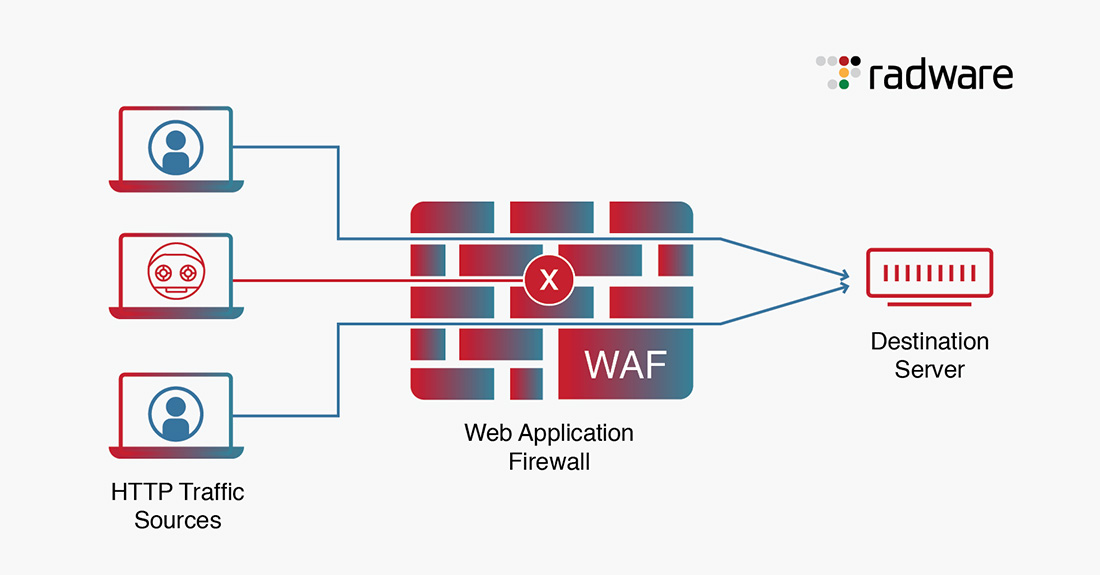
\includegraphics[width=0.8\textwidth]{waf.png}
    \caption{Web Application Firewall (WAF) protegiendo aplicaciones web}
    \label{fig:waf}
\end{figure}

\subsubsection{UFW (Uncomplicated Firewall)}
\begin{itemize}
    \item Interfaz simplificada para iptables
    \item Fácil de configurar y usar
    \item Ideal para servidores y estaciones de trabajo
\end{itemize}

\begin{figure}[H]
    \centering
    
\includegraphics[width=0.8\textwidth]{ufw.png}
    \caption{Configuración básica de UFW}
    \label{fig:ufw}
\end{figure}

\subsubsection{IPTables}
\begin{itemize}
    \item Herramienta de firewall basada en línea de comandos
    \item Permite configurar reglas de filtrado de paquetes
    \item Base para muchos firewalls modernos
\end{itemize}

\begin{figure}[H]
    \centering
    
\includegraphics[width=0.8\textwidth]{iptables.png}
    \caption{Ejemplo de configuración de IPTables}
    \label{fig:iptables}
\end{figure}

\subsubsection{Otras Herramientas}
\begin{itemize}
    \item \textbf{ClaroOS}: Solución de seguridad unificada
    \item \textbf{pfSense}: Firewall de código abierto
    \item \textbf{Snort}: Sistema de detección/prevención de intrusiones
    \item \textbf{IDS/IPS}:
    \begin{itemize}
        \item HIDS/HIPS: Basado en host
        \item NIDS/NIPS: Basado en red
    \end{itemize}
\end{itemize}

\subsection{Ataques de Fuerza Bruta}
\subsubsection{Concepto}
Ataque contra sistemas de autenticación que prueba múltiples combinaciones de credenciales hasta encontrar la correcta.

\subsubsection{Archivos Críticos en Linux}
\begin{itemize}
    \item \texttt{/etc/passwd}: Información de usuarios
    \item \texttt{/etc/shadow}: Contraseñas encriptadas
\end{itemize}

\subsubsection{Herramientas Comunes}
\begin{itemize}
    \item \textbf{John the Ripper}
    \item \textbf{Hydra}
    \item \textbf{Medusa}
\end{itemize}

\subsection{Keyloggers}
\begin{itemize}
    \item Software o hardware que registra las pulsaciones del teclado
    \item Usado para robo de credenciales
    \item Ejemplo de fraude informático
\end{itemize}

\subsection{Estándares de Seguridad}
\subsubsection{ISO/IEC 27000}
\begin{itemize}
    \item 27001: Requisitos para SGSI
    \item 27005: Gestión de Riesgos
    \item 27032: Ciberseguridad
\end{itemize}

\subsubsection{NIST Cybersecurity Framework}
Marco de trabajo para gestionar riesgos de ciberseguridad.

\section{Introducción a la Criptografía}
\subsection{Conceptos Básicos}
\begin{itemize}
    \item \textbf{Criptología}: Estudio de las comunicaciones seguras
    \item \textbf{Criptoanálisis}: Estudio de métodos para descifrar información sin autorización
    \item \textbf{Cifrado/Descifrado}: Procesos de codificación y decodificación de información
\end{itemize}

\subsection{Tipos de Criptografía}
\subsubsection{Simétrica}
\begin{itemize}
    \item Usa una sola clave secreta
    \item Ejemplo: AES, DES, 3DES
\end{itemize}

\subsubsection{Asimétrica}
\begin{itemize}
    \item Usa par de claves (pública/privada)
    \item Ejemplo: RSA, ECC
\end{itemize}

\subsubsection{Funciones Hash}
\begin{itemize}
    \item Transformación irreversible de datos
    \item Ejemplo: SHA-256, MD5
    \item Usado en integridad de datos y almacenamiento de contraseñas
\end{itemize}

\subsection{Recomendaciones de Películas}
\begin{itemize}
    \item \textit{The Imitation Game} (Sobre Alan Turing)
    \item \textit{A Beautiful Mind}
\end{itemize}

\subsection{Práctica de Laboratorio: Ataques de Fuerza Bruta}
\begin{enumerate}
    \item Configurar entorno de prueba
    \item Generar diccionario de contraseñas
    \item Ejecutar ataque usando herramientas como Hydra
    \item Analizar resultados y contramedidas
\end{enumerate}

\subsection{Conclusión}
La seguridad informática requiere un enfoque integral que combine herramientas técnicas, estándares de seguridad y concientización del usuario. La criptografía juega un papel fundamental en la protección de la información, mientras que los firewalls y sistemas de detección de intrusiones protegen los sistemas de amenazas externas e internas.


\section{Clase 5 - 8 de Mayo 2025: Ataques de Fuerza Bruta y Keyloggers}
\subsection{Objetivos de Aprendizaje}
\begin{enumerate}
    \item Comprender los ataques de fuerza bruta y sus herramientas
    \item Analizar el funcionamiento de los keyloggers
    \item Realizar prácticas de laboratorio con herramientas de seguridad
\end{enumerate}

\section{Herramientas de Ataque de Fuerza Bruta en Kali Linux}
Los ataques de fuerza bruta son intentos sistemáticos de adivinar credenciales de autenticación probando múltiples combinaciones.

\subsection{Hydra: Ataques a Protocolos de Red}
\begin{itemize}
    \item Realiza ataques de fuerza bruta contra múltiples protocolos (SSH, HTTP, FTP, etc.)
    \item Ideal para probar credenciales en servicios de red
    \item Fácil de usar y altamente configurable
\end{itemize}

\begin{figure}[H]
    \centering
    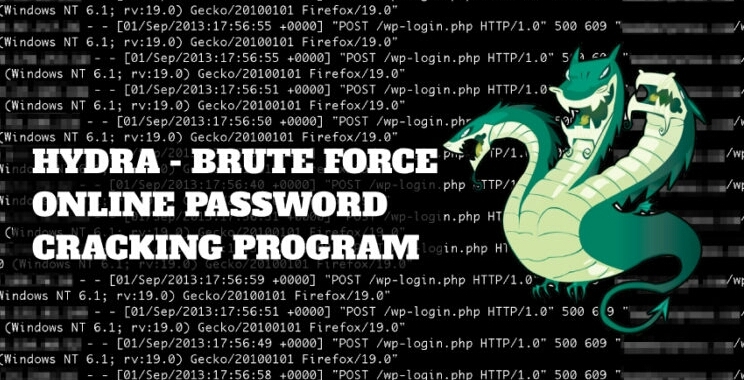
\includegraphics[width=0.9\textwidth]{hydra.png}
    \caption{Ejemplo de uso de Hydra para ataques de fuerza bruta}
    \label{fig:hydra}
\end{figure}

\subsection{John the Ripper: Descifrado de Hashes}
\begin{itemize}
    \item Especializado en descifrar contraseñas a partir de hashes
    \item Soporta múltiples algoritmos de hash
    \item Incluye modo de diccionario y ataque por fuerza bruta
\end{itemize}

\begin{figure}[H]
    \centering
    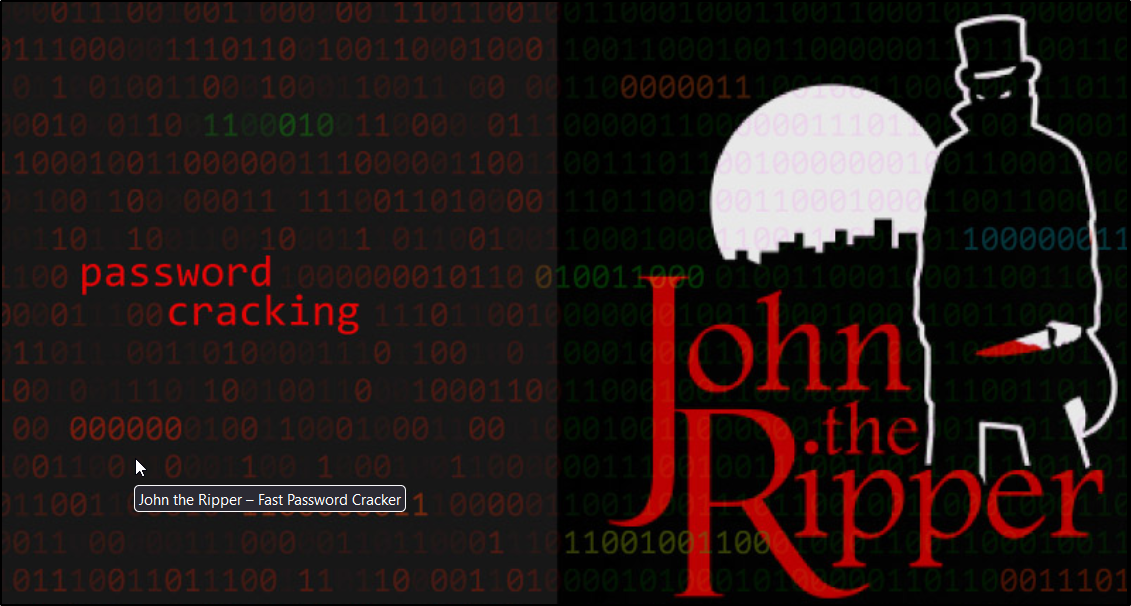
\includegraphics[width=0.9\textwidth]{john.png}
    \caption{Interfaz de John the Ripper para descifrado de contraseñas}
    \label{fig:john}
\end{figure}

\subsection{Medusa: Ataques Multi-protocolo}
\begin{itemize}
    \item Similar a Hydra, con soporte para múltiples protocolos
    \item Eficiente en el uso de recursos
    \item Permite ataques paralelos
\end{itemize}

\begin{figure}[H]
    \centering
    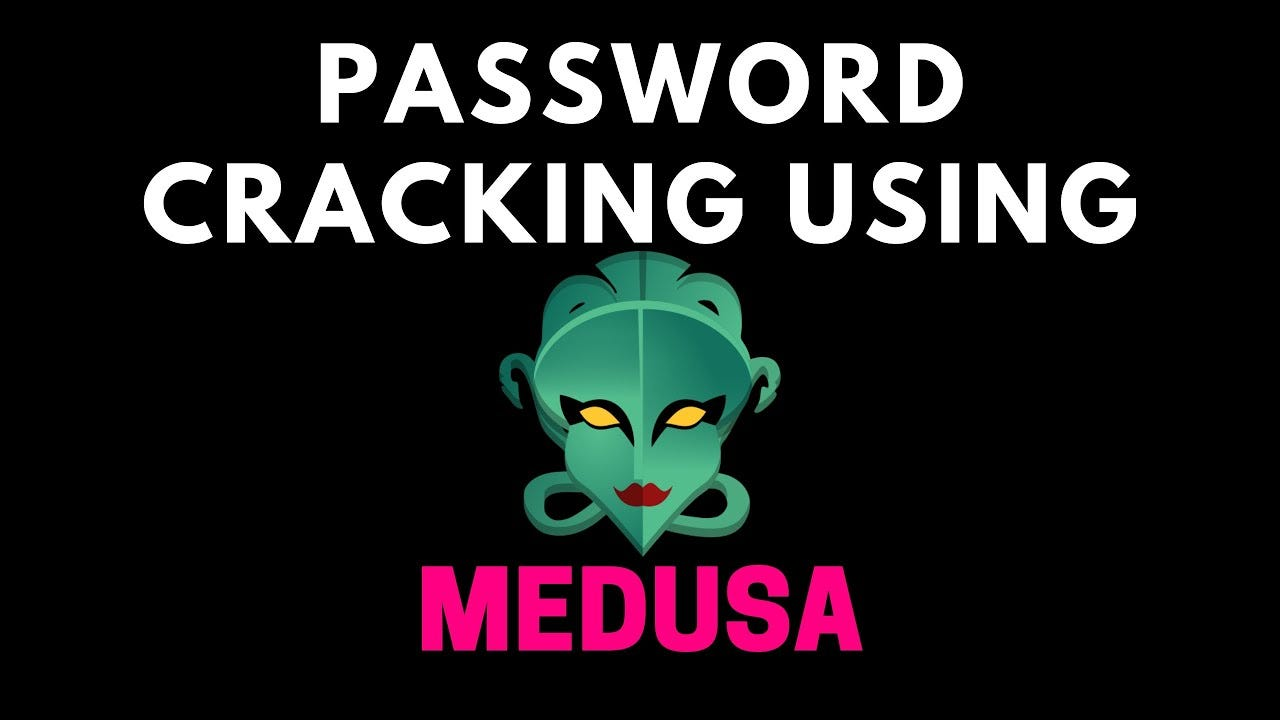
\includegraphics[width=0.9\textwidth]{medusa.png}
    \caption{Medusa en acción realizando ataques multi-protocolo}
    \label{fig:medusa}
\end{figure}

\subsection{Burp Suite: Ataques a Formularios Web}
\begin{itemize}
    \item Herramienta integral para pruebas de seguridad web
    \item Permite interceptar y modificar peticiones HTTP/HTTPS
    \item Incluye funcionalidad para ataques de fuerza bruta
\end{itemize}

\begin{figure}[H]
    \centering
    
\includegraphics[width=0.9\textwidth]{burpsuite.png}
    \caption{Burp Suite para pruebas de seguridad web}
    \label{fig:burpsuite}
\end{figure}

\subsection{Hashcat: Descifrado Avanzado de Hashes}
\begin{itemize}
    \item Herramienta avanzada para descifrado de hashes
    \item Soporta múltiples algoritmos de hash
    \item Utiliza la GPU para acelerar el proceso de descifrado
\end{itemize}

\begin{figure}[H]
    \centering
    
\includegraphics[width=0.9\textwidth]{hashcat.png}
    \caption{Hashcat para descifrado avanzado de hashes}
    \label{fig:hashcat}
\end{figure}

\section{Keyloggers}
\subsection{¿Qué es un Keylogger?}
\begin{itemize}
    \item Software o hardware que registra las pulsaciones del teclado
    \item Puede capturar contraseñas, mensajes y otra información confidencial
    \item Usado tanto para monitoreo legítimo como para actividades maliciosas
\end{itemize}

\begin{figure}[H]
    \centering
    
\includegraphics[width=0.7\textwidth]{keylogger.png}
    \caption{Ejemplo de keylogger capturando pulsaciones}
    \label{fig:keylogger}
\end{figure}

\subsection{Implicaciones de Seguridad}
\begin{itemize}
    \item \textbf{Amenaza a la privacidad}: Captura de información confidencial
    \item \textbf{Robo de identidad}: Obtención de credenciales de acceso
    \item \textbf{Impacto financiero}: Pérdidas económicas por fraude
    \item \textbf{Aspectos legales}: Uso no autorizado es penado por la ley
\end{itemize}

\section{Conclusión}
\begin{itemize}
    \item Las herramientas de fuerza bruta son efectivas contra configuraciones débiles
    \item Hydra y Medusa son versátiles para pruebas de red
    \item Los keyloggers representan una amenaza significativa a la privacidad
    \item Es esencial implementar medidas de seguridad adecuadas:
    \begin{itemize}
        \item Contraseñas fuertes
        \item Autenticación de dos factores
        \item Monitoreo de actividad sospechosa
        \item Actualizaciones de seguridad regulares
    \end{itemize}
\end{itemize}

\section{Próximos Pasos}
\begin{itemize}
    \item Practicar con herramientas de seguridad en entornos controlados
    \item Aprender sobre contramedidas y detección de ataques
    \item Explorar técnicas de hardening de sistemas
\end{itemize}

\section{Clase 6 - 13 de Mayo 2025: SGSI y Normativa ISO 27000}
\subsection{Requerimientos Funcionales de la Seguridad de la Información}
\begin{itemize}
    \item Marco normativo ISO/IEC 27000
    \item Sistema de Gestión de Seguridad de la Información (SGSI)
    \item Estándares clave:
    \begin{itemize}
        \item ISO/IEC 27001: Requisitos para SGSI
        \item ISO/IEC 27002: Código de buenas prácticas
        \begin{itemize}
            \item Control de acceso
            \item Criptografía
            \item Controles de seguridad
        \end{itemize}
    \end{itemize}
\end{itemize}

\subsection{Componentes del SGSI}
\begin{itemize}
    \item \textbf{Física}: Protección de instalaciones y equipos
    \item \textbf{Lógica}: Controles de software y acceso lógico
    \item \textbf{Procedimental}: Políticas y procedimientos
    \item \textbf{Legal}: Marco normativo aplicable
    \begin{itemize}
        \item COIP (Código Orgánico Integral Penal)
        \item Ley de Protección de Datos
        \item Ley de Comercio Electrónico
    \end{itemize}
\end{itemize}

\begin{figure}[H]
    \centering
    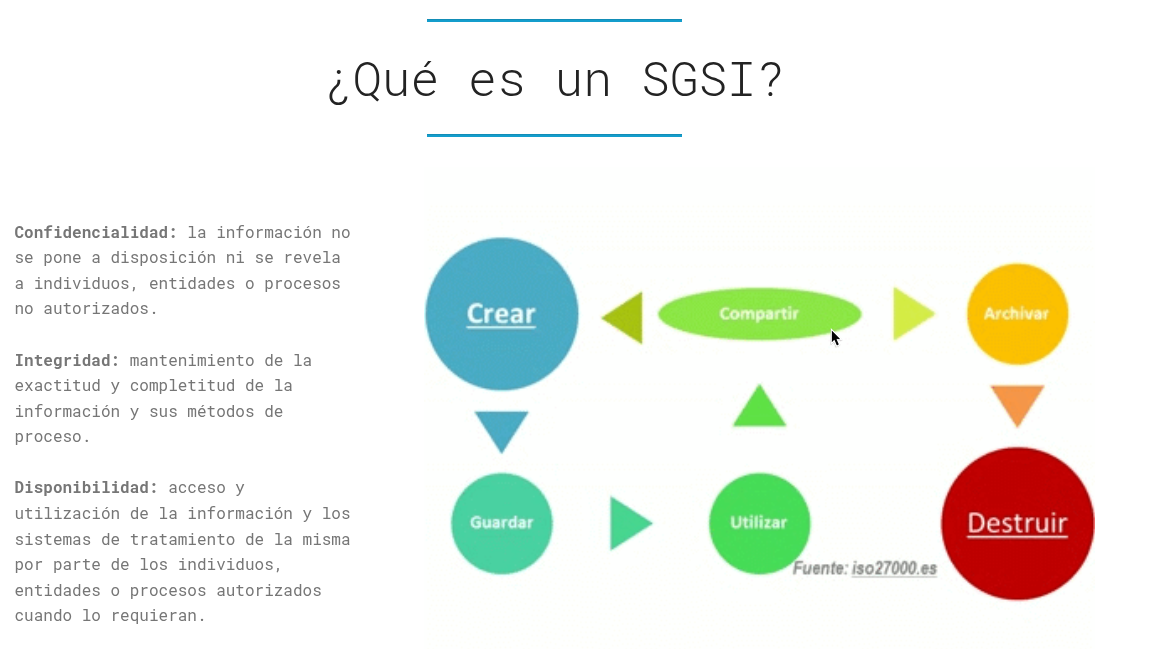
\includegraphics[width=0.9\textwidth]{sgsi.png}
    \caption{Componentes de un Sistema de Gestión de Seguridad de la Información}
    \label{fig:sgsi}
\end{figure}

\subsection{Conceptos Clave de ISO 27000}
\begin{itemize}
    \item \textbf{Organización}: Entidad que gestiona la información
    \item \textbf{Sistema}: Conjunto de elementos interrelacionados para un fin común
    \item \textbf{Activo}: Recurso con valor que requiere protección
    \item \textbf{Alcance}: Límites y cobertura del SGSI
\end{itemize}

\begin{figure}[H]
    \centering
    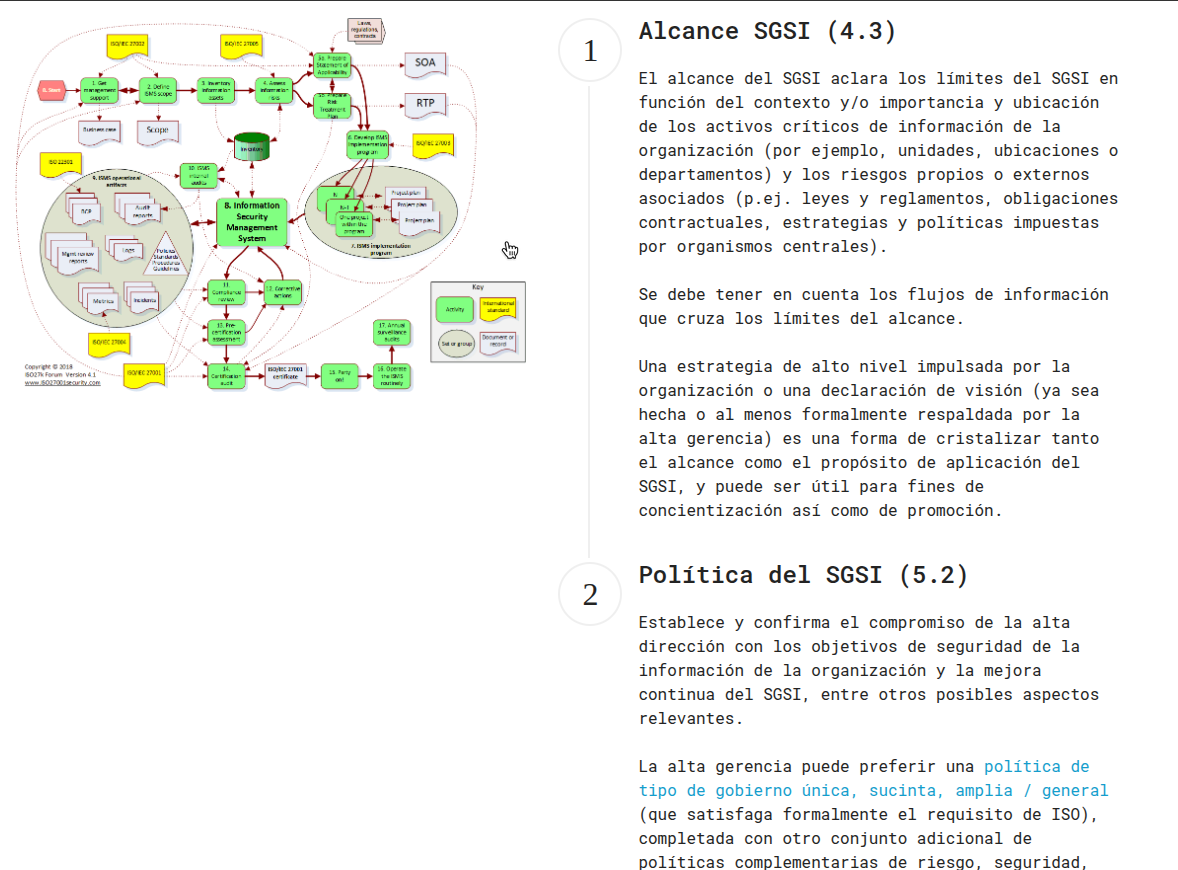
\includegraphics[width=0.9\textwidth]{alcance_sgsi.png}
    \caption{Alcance de un SGSI en una organización}
    \label{fig:alcance_sgsi}
\end{figure}

\subsection{Beneficios de Implementar un SGSI}
\begin{itemize}
    \item Protección de la información crítica
    \item Cumplimiento normativo
    \item Reducción de riesgos de seguridad
    \item Mejora continua de los procesos
    \item Ventaja competitiva
\end{itemize}

\begin{figure}[H]
    \centering
    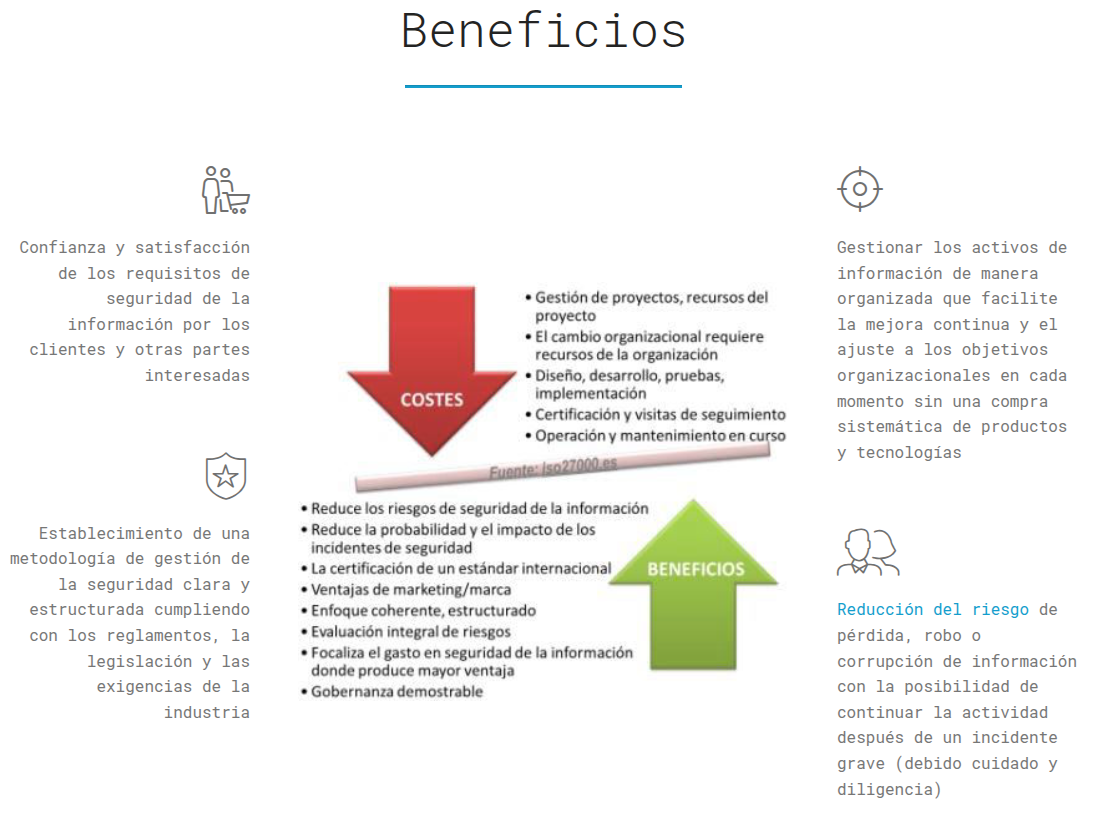
\includegraphics[width=0.9\textwidth]{sgsi_beneficio.png}
    \caption{Beneficios de implementar un SGSI basado en ISO 27001}
    \label{fig:sgsi_beneficio}
\end{figure}

\subsection{Herramientas Tecnológicas para la Seguridad}
\begin{itemize}
    \item \textbf{Mapas de Ciberataques}: Visualización de amenazas en tiempo real
    \item \textbf{Herramientas de Pruebas de Seguridad}:
    \begin{itemize}
        \item SQLMap para pruebas de inyección SQL
        \item Escáneres de vulnerabilidades
        \item Herramientas de análisis forense
    \end{itemize}
\end{itemize}

\subsection{Recursos Adicionales}
\begin{itemize}
    \item Sitio web oficial de ISO 27000: \url{https://www.iso27000.es/}
    \item Documentación oficial de ISO/IEC 27001 e ISO/IEC 27002
    \item Guías de implementación de SGSI
\end{itemize}

\subsection{Conclusión}
\begin{itemize}
    \item La implementación de un SGSI basado en ISO 27001 es fundamental para la gestión efectiva de la seguridad de la información
    \item La norma proporciona un enfoque sistemático para gestionar la información confidencial
    \item La adopción de estas normas ayuda a las organizaciones a proteger sus activos de información
\end{itemize}

\subsection{Próximos Pasos}
\begin{itemize}
    \item Estudiar los requisitos específicos de ISO 27001
    \item Analizar casos de estudio de implementación de SGSI
    \item Explorar herramientas para la gestión de seguridad de la información
\end{itemize}


\section{Clase 7 - 15 de Mayo 2025: Especificación de Requisitos de Seguridad}

\subsection{Objetivo de Aprendizaje}
\begin{itemize}
    \item Especificación de Requerimientos de seguridad del Software
    \begin{itemize}
        \item NIST
        \item CYBERSECURITY
        \item Framework
    \end{itemize}
    \item Ensayo argumentativo
    \begin{itemize}
        \item Cyber Threats Word Maps
        \item Mejorar la escritura
    \end{itemize}
    \item Práctica de laboratorio SQLMap
\end{itemize}

\subsection{Reflexión}
F= M+V+CA (Alberto Meraní)

Felicidad = F

Metas = M

Vínculos = V

Cualidades Afectivas = CA

→ Es una decisión

Metas → Soñarlas, dibujarlas acciones

Para ello podemos hacer un metagrama con los siguientes campos:

\begin{figure}[H]
\centering
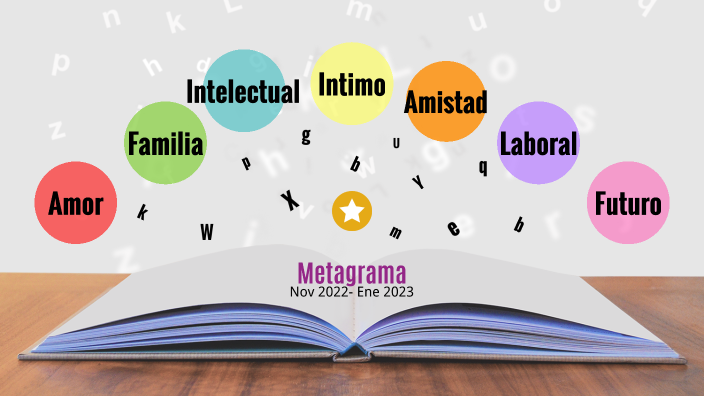
\includegraphics[width=0.9\textwidth]{metagrama.png}
\caption{Metagrama para la planificación de metas}
\label{fig:metagrama}
\end{figure}

\subsection{Consejos de Edición}
\subsubsection{Escritura de párrafos}
\begin{itemize}
    \item Coherencia y secuencialidad en los párrafos (utilizar conectores gramaticales)
    \item Evitar el uso de adjetivos calificativos
    \item Evitar errores ortográficos
    \item Evitar el uso de adverbios
\end{itemize}

\section{Clase 8 - 20 de Mayo 2025: Especificación de Requisitos de Seguridad}
\subsection{Introducción}
En el desarrollo de software seguro, los requisitos de seguridad son la base para construir aplicaciones confiables. Vamos a explorar los estándares clave y cómo implementar estos requisitos de manera efectiva.

\subsubsection{Estándares Clave}
\begin{center}
\begin{tabular}{|l|p{10cm}|}
\hline
\textbf{Estándar} & \textbf{Descripción} \\ \hline
ISO 27000 & Familia de normas para la gestión de seguridad de la información \\
NIST & Marco de ciberseguridad del Instituto Nacional de Estándares y Tecnología \\
OWASP & Proyecto de seguridad de aplicaciones web abierto \\ \hline
\end{tabular}
\end{center}

\subsection{Requisitos Esenciales de Seguridad}

\subsubsection{1. Autenticación y Autorización}
\begin{center}
\fbox{\begin{minipage}{0.9\textwidth}
\textbf{Ejemplo Práctico}: Un sistema bancario requiere autenticación de dos factores para transacciones superiores a \$1,000.
\end{minipage}}
\end{center}

\begin{itemize}
    \item \textbf{MFA}: Implementación de autenticación multifactor
    \item \textbf{RBAC}: Control de acceso basado en roles
    \item \textbf{JWT}: Uso de tokens seguros para sesiones
\end{itemize}

\subsubsection{2. Validación de Entrada}
\begin{verbatim}
def validar_entrada(usuario):
    # Validación por lista blanca
    caracteres_permitidos = set("abcdefghijklmnopqrstuvwxyz0123456789_-")
    if not all(c in caracteres_permitidos for c in usuario):
        raise ValueError("Caracteres no permitidos")
    return usuario
\end{verbatim}

\subsubsection{3. Seguridad en la Comunicación}
\begin{center}
\begin{tabular}{|l|p{8cm}|}
\hline
\textbf{Protocolo} & \textbf{Uso Seguro} \\ \hline
HTTP & No recomendado \\
HTTPS & Obligatorio para todo tipo de comunicación segura \\
SFTP & Para transferencia segura de archivos \\
WPA3 & Para redes inalámbricas seguras \\ \hline
\end{tabular}
\end{center}

\subsection{OWASP Top 10: Amenazas Principales}
1. \textbf{Inyección} (SQL, NoSQL, OS, LDAP)
2. \textbf{Autenticación Rota}
3. \textbf{Exposición de Datos Sensibles}
4. \textbf{Entidades Externas XML (XXE)}
5. \textbf{Control de Acceso Roto}
6. \textbf{Configuración de Seguridad Incorrecta}
7. \textbf{Cross-Site Scripting (XSS)}
8. \textbf{Deserialización Insegura}
9. \textbf{Componentes Vulnerables}
10. \textbf{Registro y Monitoreo Insuficientes}

\subsection{Práctica de Laboratorio: OWASP ZAP}
1. Instalar OWASP ZAP
2. Configurar el navegador para usar ZAP como proxy
3. Analizar una aplicación web
4. Identificar vulnerabilidades
5. Generar reporte de hallazgos

\begin{figure}[H]
\centering
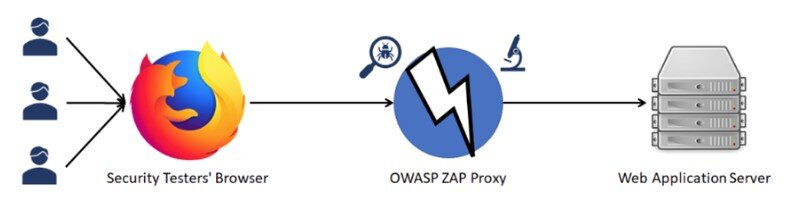
\includegraphics[width=0.9\textwidth]{owasp_zap.png}
\caption{Interfaz de OWASP ZAP para pruebas de seguridad}
\label{fig:owasp_zap}
\end{figure}

\subsection{Checklist de Seguridad}
\begin{itemize}
    \item[--] ¿Se validan todas las entradas del usuario?
    \item[--] ¿Se implementa el principio de mínimo privilegio?
    \item[--] ¿Los datos sensibles están cifrados?
    \item[--] ¿Existen registros de auditoría suficientes?
    \item[--] ¿Se actualizan regularmente las dependencias?
\end{itemize}

\subsection{Recursos Adicionales}
\begin{itemize}
    \item OWASP: \url{https://owasp.org/}
    \item NIST: \url{https://csrc.nist.gov/}
    \item ISO 27001: \url{https://www.iso.org/isoiec-27001}
\end{itemize}

\subsection{Conclusión}
La seguridad del software no es un producto, sino un proceso continuo. La implementación de estos requisitos debe ser parte integral del ciclo de vida del desarrollo de software, no una ocurrencia tardía.
\textit{"La seguridad siempre es excesiva hasta que ya no es suficiente."}


\section{Clase 9 - 22 de Mayo 2025: Análisis de Amenazas y Vulnerabilidades}

\subsection{Objetivos de aprendizaje}
\begin{enumerate}
    \item Análisis de las amenazas y vulnerabilidades más comunes
    \begin{enumerate}
        \item Magerit
        \item OWASP
        \item EGSI
    \end{enumerate}
    \item Práctica de laboratorio de análisis de vulnerabilidades OWASP-ZAP
\end{enumerate}


\subsection{Reflexión: Zona de Confort}

La zona que usted conoce aquí no requiere más esfuerzo, pero ¿a cambio de qué?

Al salir de esa zona de confort, se entra a una zona de pánico. 

Le llaman la zona de pánico porque se desconocen las cosas, pero si usted sigue avanzando, poco a poco esa zona de pánico se convierte en zona de aprendizaje. Se va saliendo de la zona de pánico, hasta que se llega a una tercera zona, que ahora tiene dos pisos, y que se llama la zona de descubrimiento, la zona de crecimiento. 

\begin{figure}[H]
\centering
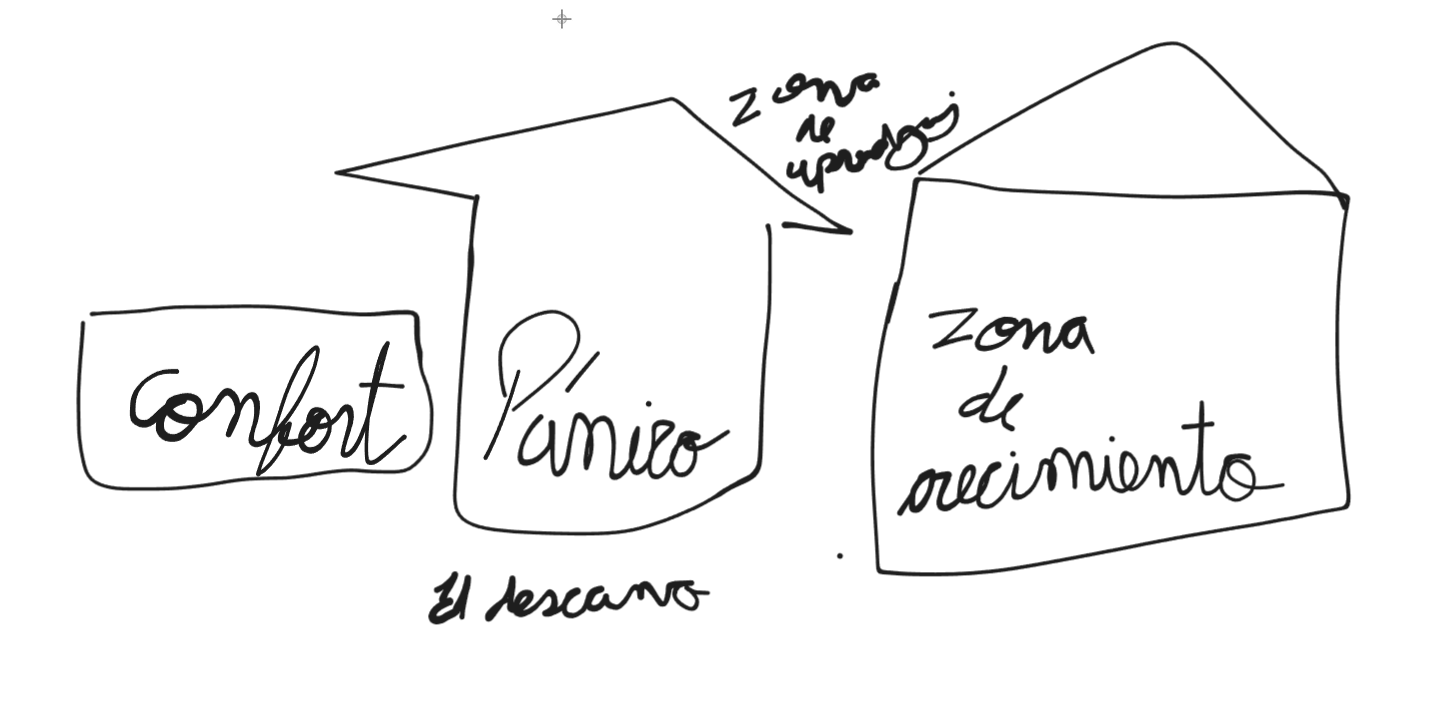
\includegraphics[width=0.9\textwidth]{confort.png}
\caption{Modelo de zonas de desarrollo personal}
\label{fig:confort}
\end{figure}

\subsection{Mia: Aprendizaje Activo}

Para aprender realmente, es mejor hacer las cosas por uno mismo, equivocarse y ahí aprender. 

El verdadero aprendizaje no es copiar y pegar, sino cuestionarse lo que se hace, lo que uno cree y la manera en que uno aprende. Esa curiosidad y el darle espacio a la experimentación es la mejor manera de aprender. Con la práctica se aprende, y a través de la práctica es como realmente se consolida el conocimiento.

\subsection{Marco Teórico: Amenazas y Vulnerabilidades}

\begin{itemize}
    \item \textbf{Amenaza} (si no tiene backups o respaldos) + \textbf{vulnerabilidades} = \textbf{riesgo}
    \item \textbf{Amenazas Naturales}:
    \begin{itemize}
        \item Fuego
        \item Erupción volcánica
        \item Movimientos telúricos
    \end{itemize}
    \item \textbf{Amenazas}: Causa potencial de un incidente que puede causar daños en un sistema personal, institución o país
    \begin{itemize}
        \item Humanas
        \begin{itemize}
            \item Intencionales (ej. incendios provocados)
            \item No intencionales (por omisión o negligencia)
        \end{itemize}
    \end{itemize}
    \item \textbf{Procedimientos}:
    \begin{itemize}
        \item Técnicas (bugs, troyanos, spyware, gusanos)
        \item Tecnologías (cortocircuitos, obsolescencia, incumplimiento de normas)
    \end{itemize}
    \item \textbf{Vulnerabilidades}: Debilidad que puede ser explotada por un ciberataque interno o externo
\end{itemize}

\subsubsection{Ejemplos de vulnerabilidades comunes}
\begin{enumerate}
    \item Mal funcionamiento y herramientas sin licencia
    \item Gestión inadecuada de red o falla en los enlaces de comunicación
    \item Destrucción de registros y respaldo irregular
    \item Acceso a información restringida y compartir credenciales
    \item Falta de monitoreo de red y ataques a páginas publicadas
    \item Suspensión del servicio y actualización de parches del software base
    \item Falta de monitoreo y ciberataques
\end{enumerate}

\begin{figure}[H]
\centering
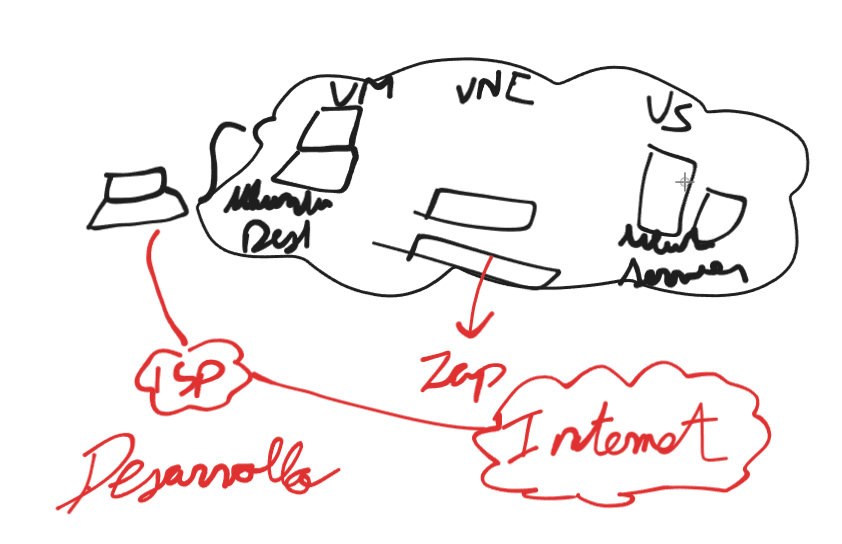
\includegraphics[width=0.9\textwidth]{dibujo_practica.png}
\caption{Diagrama de análisis de riesgos}
\label{fig:dibujo_practica}
\end{figure}

\subsection{ESQUEMA GUBERNAMENTAL DE SEGURIDAD DE LA INFORMACIÓN (EGSI)}

Puede encontrar más información en: \url{https://www.gobiernoelectronico.gob.ec/egsi/}

\subsection{Avance de la Práctica de laboratorio 5: Análisis de vulnerabilidades con OWASP-ZAP}

\subsubsection{Objetivo de aprendizaje}
\begin{enumerate}
    \item Comprender el funcionamiento de las herramientas de análisis de vulnerabilidades OWASP
    \item Aprender a utilizar OWASP-ZAP para identificar amenazas y vulnerabilidades
    \item Realizar escaneos activos y pasivos para detectar vulnerabilidades comunes en aplicaciones web
\end{enumerate}

\subsection{Marco teórico}

\subsubsection{OWASP}
Open Web Application Security Project (OWASP) es una comunidad abierta dedicada a permitir que las organizaciones desarrollen, adquieran y mantengan aplicaciones confiables.

\subsubsection{OWASP-ZAP (Zed Attack Proxy)}
Herramienta de seguridad para aplicaciones web que ayuda a encontrar vulnerabilidades como:
\begin{itemize}
    \item Inyección SQL
    \item Cross-Site Scripting (XSS)
    \item Fugas de información
    \item Autenticación insegura
\end{itemize}

\begin{figure}[H]
\centering
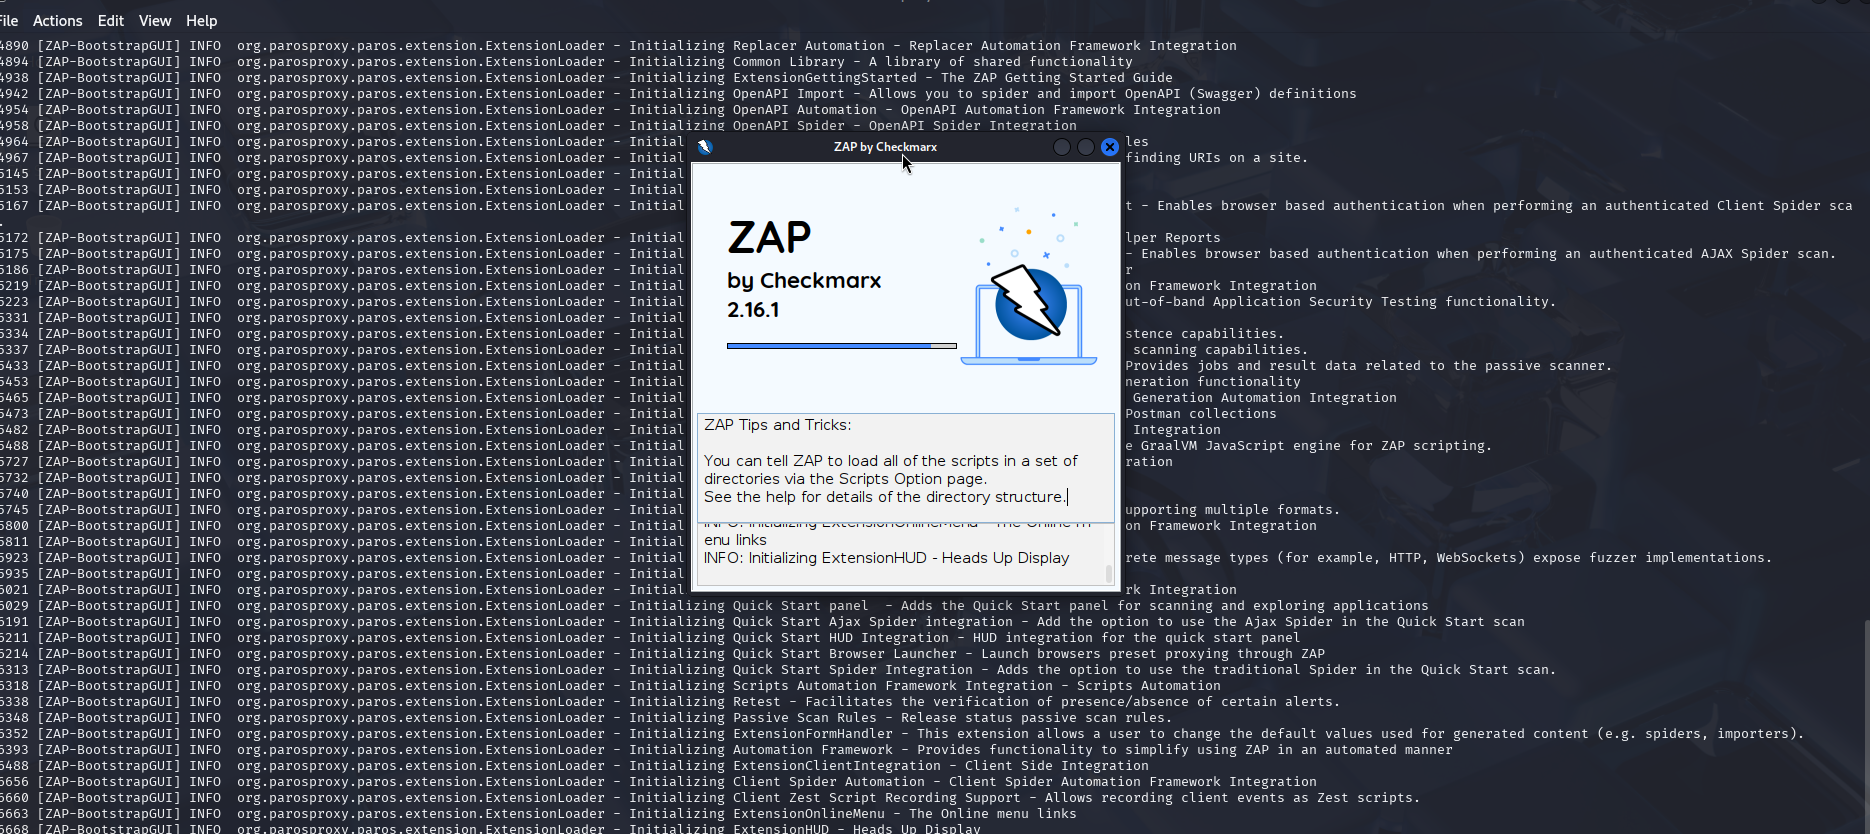
\includegraphics[width=0.9\textwidth]{zap_inicando.png}
\caption{Interfaz de inicio de OWASP-ZAP}
\label{fig:zap_inicio}
\end{figure}

\begin{figure}[H]
\centering
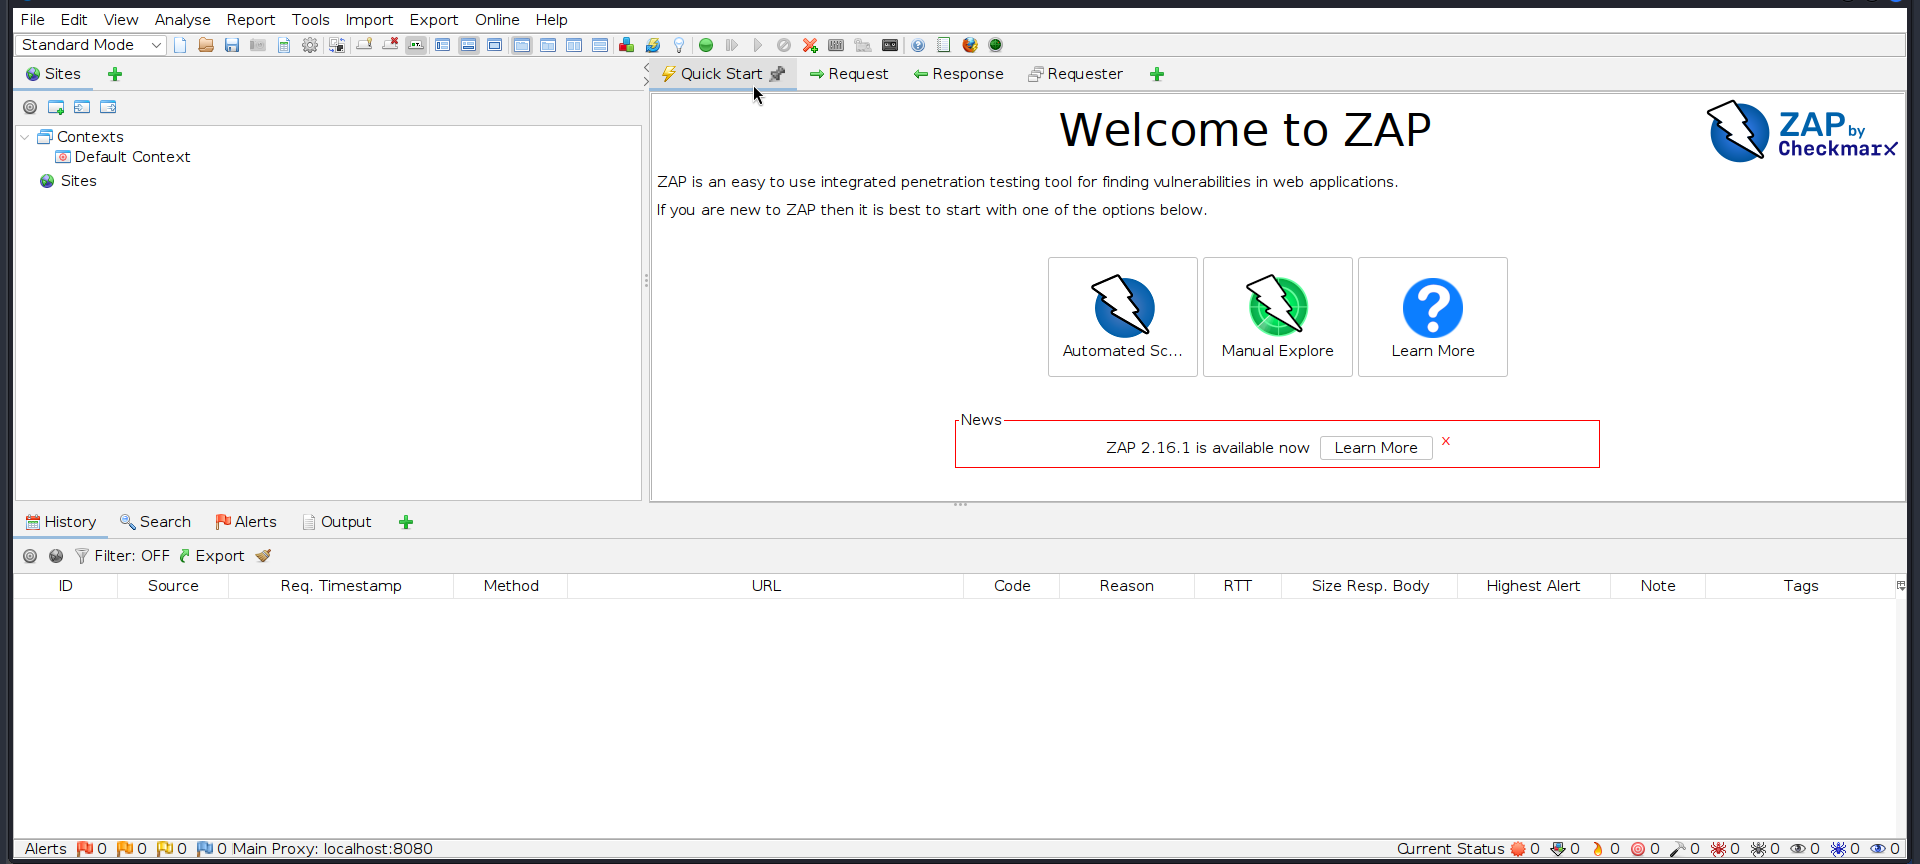
\includegraphics[width=0.9\textwidth]{zap_interfaz.png}
\caption{Vista general de la interfaz de OWASP-ZAP}
\label{fig:zap_interfaz}
\end{figure}

\end{document}